\documentclass[12pt,a4paper,twoside, openright]{scrartcl} 
\usepackage[scaled]{helvet}
\usepackage[italian]{babel}
\usepackage[utf8]{inputenc}
\usepackage[T1]{fontenc}
\usepackage{fancyhdr}
\usepackage{lastpage}
%\usepackage{ifthen}
\usepackage{amsmath,amsfonts,amsthm}
\usepackage{sfmath}
\usepackage{sectsty}
\usepackage{listings}
\lstset{language=Matlab,frame=single,numbers=left}
\usepackage{graphicx}
\usepackage{float}
\usepackage{amsthm}
\addtokomafont{caption}{\small}
\setkomafont{captionlabel}{\normalfont\bfseries}
\let\oldtabular\tabular
\renewcommand{\tabular}{\sffamily\oldtabular}
%\KOMAoptions{abstract=true}
\renewcommand\familydefault{\sfdefault}
\renewcommand{\arraystretch}{1.1}
\newcommand{\horrule}[1]{\rule{\linewidth}{#1}}
\setlength{\textheight}{230mm}
\allsectionsfont{\centering \normalfont\scshape}
\let\tmp\oddsidemargin
\let\oddsidemargin\evensidemargin
\let\evensidemargin\tmp
\reversemarginpar
\setlength\parindent{0pt}
\usepackage{caption}
\usepackage{subfig}
\newcommand{\thetap}{\dot{\theta}}
%\graphicspath{{Immagini/}}
\fancypagestyle{plain}
{
	\renewcommand{\headrulewidth}{0pt}%
	\renewcommand{\footrulewidth}{0.5pt}
	\fancyhf{}%
	\fancyfoot[R]{\emph{\footnotesize Page \thepage\ of \pageref{LastPage}}}%
	\fancyfoot[C]{\emph{\footnotesize Leonardo Soccio}\\ \emph{\footnotesize 0251992}}%
}
%\author{Leonardo Soccio}
\title{Analisi Fisica del progetto}
\date{\vspace{-5ex}}
%\date{}  % Toggle commenting to test

\begin{document}
	\pagestyle{plain}
	\maketitle
	Il sistema può essere ricondotto a un asta vincolata nel punto  $O$ e a un disco vincolato in $D$ che viene messo in moto da un motore.\\ 
	Lo scopo dell'analisi è capire come varia l'angolo $\theta$ con la verticale in modo tale da poterlo controllare controllando il motore che muove il disco.
	\section{Rappresentazione del sistema}
		\begin{figure}[H]
			\begin{center}
			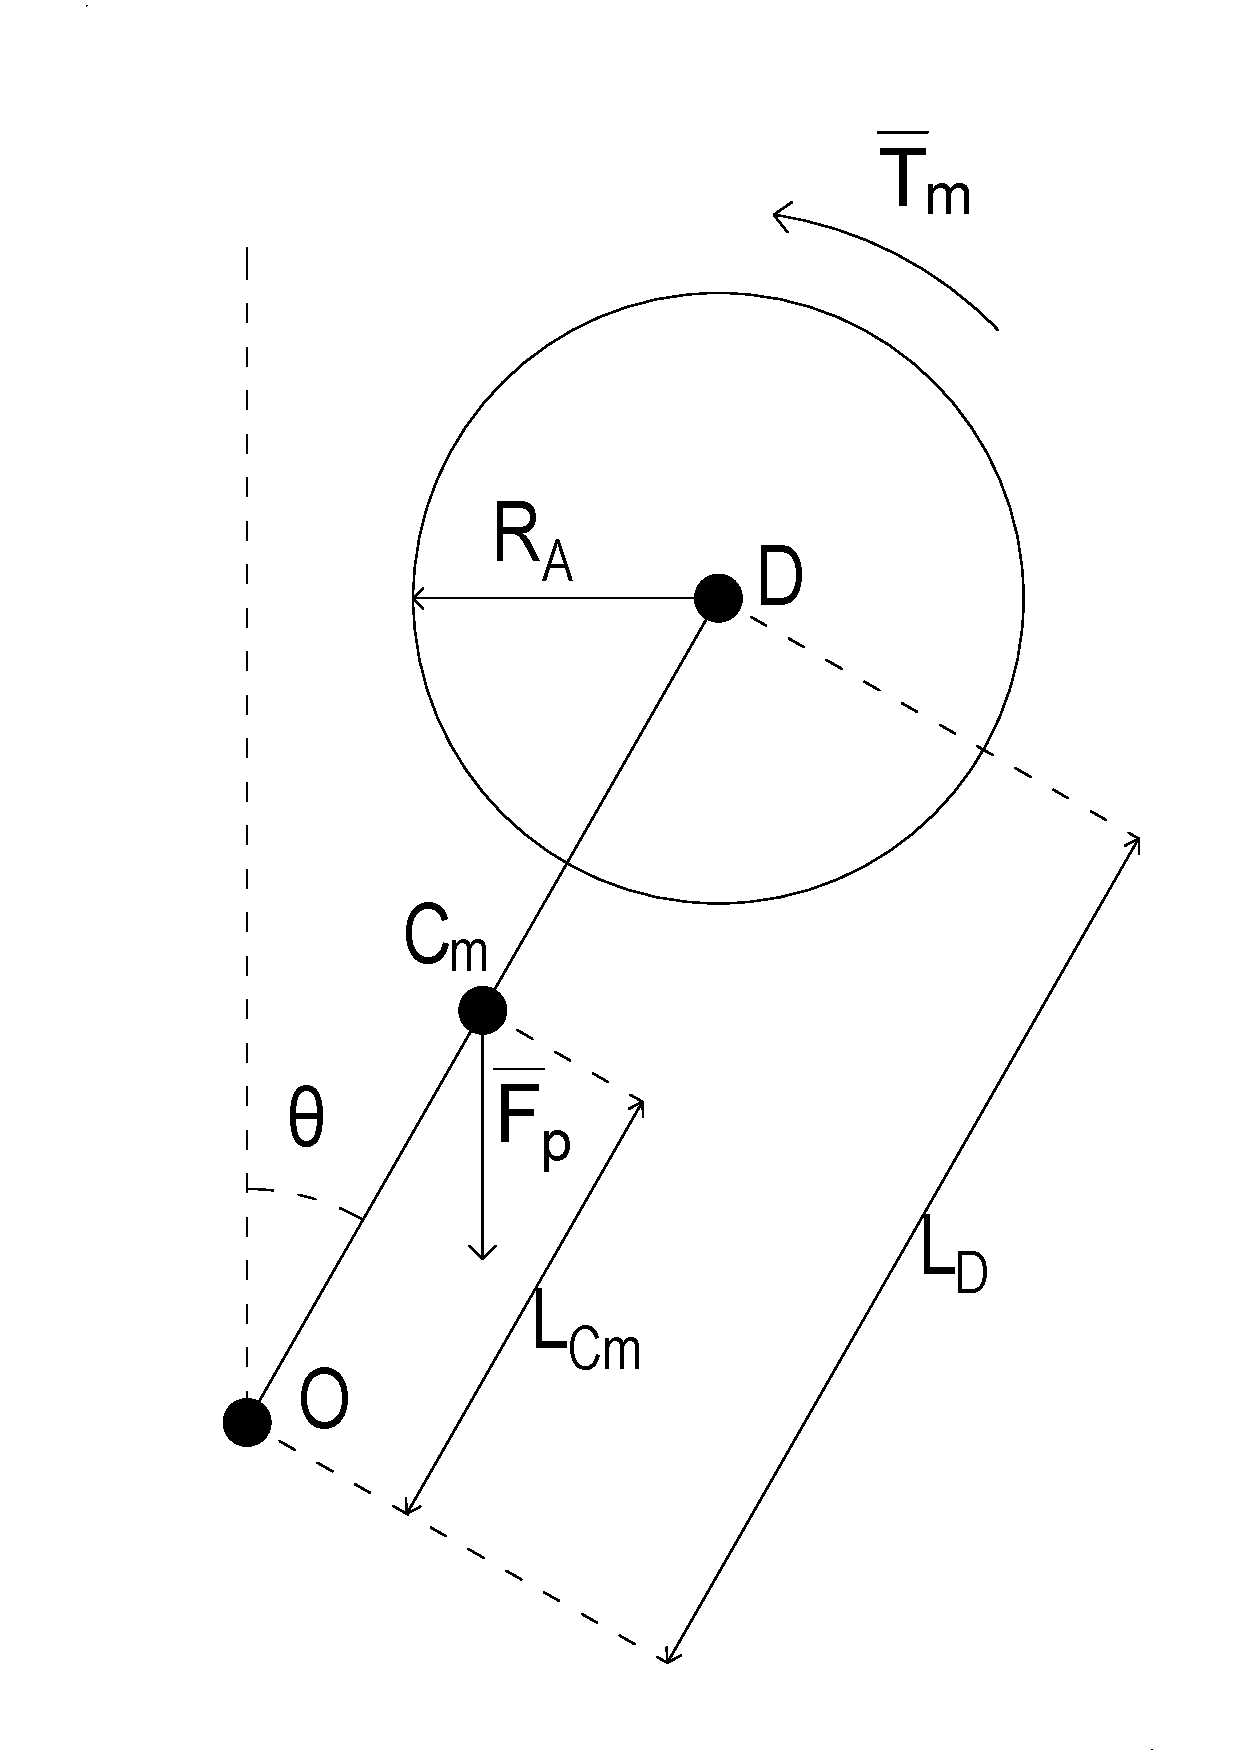
\includegraphics[height=8cm]{Figura1}
			\end{center}
			%\caption{Schema del pendolo inverso}
			\label{fig:struttura}
		\end{figure}
	Le caratteristiche del sistema sono:
	\begin{itemize}
	\item $O$ è il punto in cui il sistema è vincolato;
	\item $\theta$ è l'angolo di inclinazione rispetto la verticale dell'asta;
	\item $C_m$ è il centro di massa dell'intero sistema, considerando anche la ruota;
	\item $L_{C_m}$ è la distanza del centro di massa $C_m$ dal polo $O$; 
	\item $D$ è il punto in cui è vincolata la ruota e il motore(non rappresentato);
	\item $L_D$ è la distanza del punto $D$ dal polo $O$; 
	\item $\overline{F}_p$ è la forza peso totale agente sul sistema, considerata applicata nel centro di massa;
	\item $ \overline{\tau}_m$ è la coppia che il motore fornisce al sistema;
	\item $I_t$ è l'inerzia totale del sistema rispetto il polo $O$;
	\item $I_d$ è l'inerzia del disco rispetto il punto $D$;
	\end{itemize}
	Per l'analisi considererò trascurabili tutti gli attriti e considerero la coppia del motore linearmente legata alla tensione.\\
	Per la seconda equazione cardinale della meccanica si avrà che:
	\begin{equation}
	\label{eqn:1}
	I_t\thetapp=F_p L_{C_m}\sin(\theta)- \tau_m
	\end{equation}
	per chiarezza nell'esposizione pongo $F_p L_{C_m}=K_{mgl}$ in quanto valore costante.
	Inoltre siamo a conoscenza di due relazioni:
	 \begin{align}
	 	\tau_m &=I_d \dot{w}_{inerziale} \label{eqn:2} \\
	 	\tau_m &=kV(t) \label{eqn:3}
	 \end{align}
	Dove:
	\begin{itemize}
			\item $\dot{w}_{inerziale}$ è la velocità angolare assoluta del disco;
			\item $k$ è una costante che dipende dal motore usato;
			\item $V(t)$ è la tensione variabile ai capi del motore-
	\end{itemize}
	Infine dai moti relativi vale che:
	\begin{equation}
		\label{eqn:4}
			w_{inerziale}=\thetap+w_R 
	\end{equation}
	sostituendo la \ref{eqn:3} nella \ref{eqn:1}:
	\begin{equation}
		\label{eqn:5}
	 		I_t\thetapp=K_{mgl}\sin(\theta)-kV(t)
	\end{equation}
	quindi, approssimando per piccoli angoli ($\sin(\theta)\approx \theta$):
	\begin{equation}
		\label{eqn:6}
	 		\thetapp=\frac{K_{mgl}}{I_t}\theta-\frac{k}{I_t}V(t)
	\end{equation}
 	Inoltre sostituendo la \ref{eqn:4} nella \ref{eqn:2} si ottiene che :
	\begin{equation}
		\label{eqn:7}
			\tau_m =I_d(\thetapp+\dot w_R) 
	\end{equation}
	Si sostituisce poi nella \ref{eqn:3}:
	\begin{equation}
		\label{eqn:8}
			I_d(\thetapp+\dot w_R)=kV(t) 
	\end{equation}
	E quindi:
	\begin{equation}
		\label{eqn:9}
			\dot w_R=-\thetapp+\frac{k}{I_d}V(t) 
	\end{equation}
Cioè abbiamo ottenuto due equazioni differenziali la \ref{eqn:6} e \ref{eqn:9}, dipendenti dalla tensione del motore:
	\begin{equation}
		\label{sis:1}
			\begin{cases}
				\thetapp=\frac{K_{mgl}}{I_t}\theta-\frac{k}{I_t}V(t)\\
				\dot w_R=-\thetapp+\frac{k}{I_d}V(t) 
			\end{cases}
	\end{equation}
Inoltre $\theta$ e $w_R$ sono grandezze che possiamo misurare nel tempo e quelle misurate le chiamerò : $w_{R0}$ e $\theta_0$
\section{Osservazioni e domande}
	Siamo arrivati a un sistema differenziale che può essere integrato e che quindi ci permette di calcolare la variazione di $\theta$ nel tempo in funzione della tensione. Ora quello che mi chiedo è:
Cosa dobbiamo fare quindi per riportare a 0 l'angolo?  prendiamo in input i valori, soprattutto l'angolo. però come calcolare la funzione tensione in modo che quell'angolo vada a 0?
perchè integrando il sistema conosciamo cosa fa $\theta$ ma bisogna invece capire come far variare la tensione al variare casuale di $\theta$. Avete idee? 
\end{document}
